\section{Benchmark operation}
% \addcontentsline{toc}{section}{Benchmark operation}
\subsection{Different Matrix-Multiplication functions}

     \paragraph*{}
     In order to achieve theoretical times (those associated with the previous expression), we need to 
     choose which mathematical operator will be used in the benchmarks. To begin, a common operator 
     will be used: matrix multiplication.

     \paragraph{}
     The next point to address is which matrix multiplication function we will use; the options are 
     either Julia's native function, associated with the \textbf{*} operator (\texttt{matrix\_multiplication}), or manually 
     constructing a custom matrix multiplication function (\texttt{my\_matrix\_multiplication}, \texttt{my\_efficient\_matrix\_multiplication}). To compare which of these options performs better, the number 
     of GFLOPS (y-axis) will be plotted for different values of N, the dimension of the matrices to 
     be multiplied (x-axis).

\vspace*{0.5cm}

\lstinputlisting[language=Julia]{code/dot_func_comparison-v2.jl}

\vspace*{1cm}

\paragraph{} The results of running this code are shown in the following two figures; in the first 
one (Figure \ref{fig:1-dotproductcomparison}) you can see the difference between the functions \texttt{my\_matrix\_multiplication} and 
\texttt{my\_efficient\_matrix\_multiplication}. This difference lies in the transpose of the B matrix. 
This is because in Julia matrices are stored in column order, that is, consecutive columns are stored 
contiguously in memory. Therefore, when iterating over the elements of a matrix, it is more efficient 
to traverse it by columns than by rows.

\begin{figure}[h]
     \begin{center}
         % Recommended preamble:
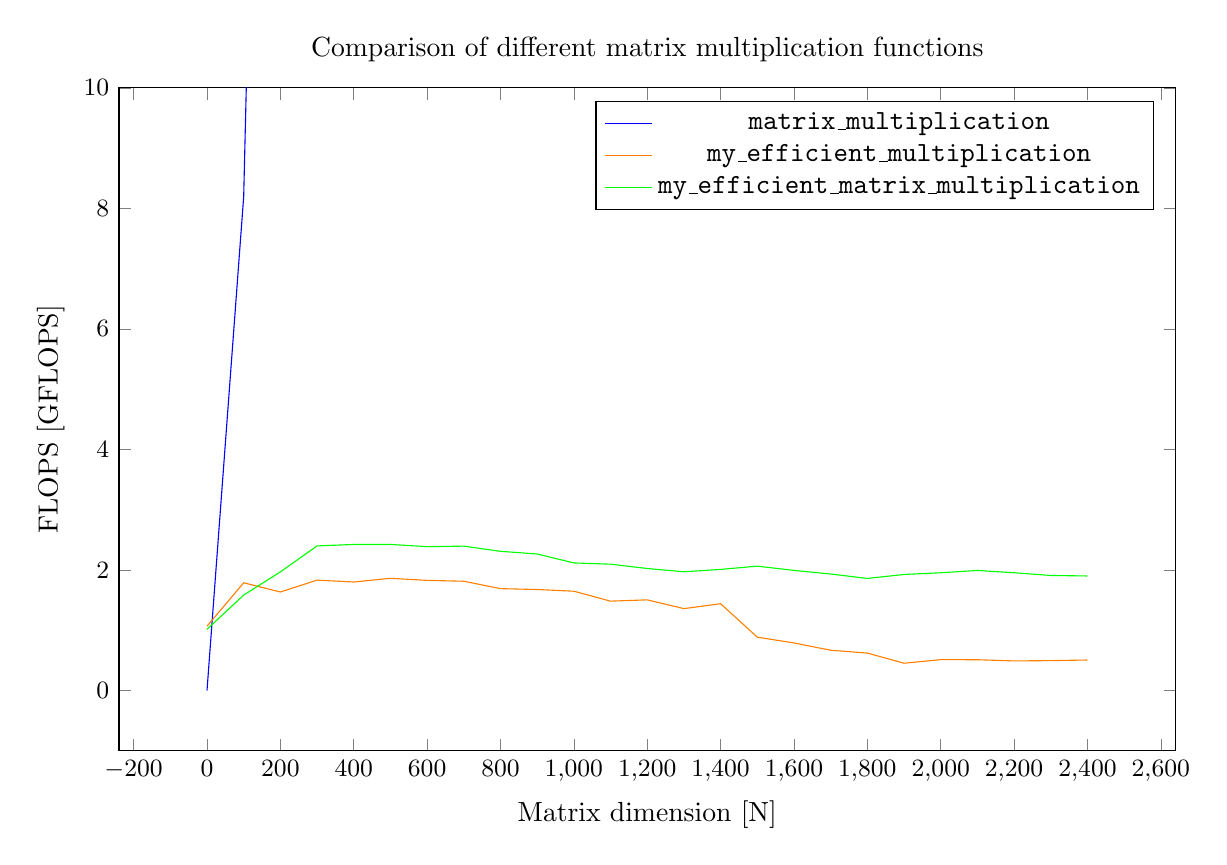
\begin{tikzpicture}
\begin{axis}[width={15cm}, height={10cm}, xlabel={Matrix dimension [N]}, ylabel={FLOPS [GFLOPS]}, title={Comparison of different matrix multiplication functions}, legend={north east}, ymax={10},    scaled ticks=false,   % Prevents scientific notation or compression in the ticks
    xticklabel style={/pgf/number format/fixed},  % Ensures tick labels are printed in a fixed format without rounding
    xticklabel style={/pgf/number format/precision=0},  % Rounds the numbers to integers to avoid crowding
    ticklabel style = {font=\small},  % Reduces the size of the tick labels to prevent overlap
    ]
    \addplot[no marks, blue]
        table[row sep={\\}]
        {
            \\
            0.0  0.0023079523961738765  \\
            100.0  8.194097294901313  \\
            200.0  33.72498893859692  \\
            300.0  63.67891003491642  \\
            400.0  83.20933205921395  \\
            500.0  121.0965154318156  \\
            600.0  114.15410635879024  \\
            700.0  148.78480554332117  \\
            800.0  128.77979771936313  \\
            900.0  46.69649114974178  \\
            1000.0  149.39668260804913  \\
            1100.0  185.67318648613312  \\
            1200.0  139.70476585037548  \\
            1300.0  140.825722756572  \\
            1400.0  157.08443564188434  \\
            1500.0  189.98083748640684  \\
            1600.0  201.73749401185015  \\
            1700.0  238.16347699049706  \\
            1800.0  184.7190920582196  \\
            1900.0  236.60746961674465  \\
            2000.0  189.07665556113673  \\
            2100.0  208.35783211953395  \\
            2200.0  211.28693733594844  \\
            2300.0  220.6979894130633  \\
            2400.0  185.3414228183199  \\
        }
        ;
    \addplot[no marks, orange]
        table[row sep={\\}]
        {
            \\
            0.0  1.0689470871191875  \\
            100.0  1.7891119566042895  \\
            200.0  1.6363952973381144  \\
            300.0  1.833138380472606  \\
            400.0  1.8019750452823982  \\
            500.0  1.8633233611285047  \\
            600.0  1.829149502012656  \\
            700.0  1.814902720882529  \\
            800.0  1.691969911709576  \\
            900.0  1.67758644720142  \\
            1000.0  1.649210445467428  \\
            1100.0  1.4844659134712057  \\
            1200.0  1.50570400213252  \\
            1300.0  1.36048195288819  \\
            1400.0  1.441815509625949  \\
            1500.0  0.8870844660154257  \\
            1600.0  0.7907230876381947  \\
            1700.0  0.6699917469778933  \\
            1800.0  0.622945715952708  \\
            1900.0  0.4545396698327844  \\
            2000.0  0.5141040422999137  \\
            2100.0  0.5125469619014145  \\
            2200.0  0.49265788054693666  \\
            2300.0  0.497771062036038  \\
            2400.0  0.5078183160369875  \\
        }
        ;
    \addplot[no marks, green]
        table[row sep={\\}]
        {
            \\
            0.0  1.017293997965412  \\
            100.0  1.5855298659744814  \\
            200.0  1.9699571431686191  \\
            300.0  2.4009089137903974  \\
            400.0  2.424738077028364  \\
            500.0  2.4250974800940805  \\
            600.0  2.3888349809526823  \\
            700.0  2.3969416901613645  \\
            800.0  2.3114564185518116  \\
            900.0  2.2665805230657363  \\
            1000.0  2.1183366990174863  \\
            1100.0  2.098103432813833  \\
            1200.0  2.02596145383276  \\
            1300.0  1.9715949457443354  \\
            1400.0  2.010909758662662  \\
            1500.0  2.065411932336678  \\
            1600.0  1.9941957000538721  \\
            1700.0  1.9348035190308683  \\
            1800.0  1.86114085663287  \\
            1900.0  1.9272390772083445  \\
            2000.0  1.9553976471457613  \\
            2100.0  1.993427896663581  \\
            2200.0  1.9556294361633033  \\
            2300.0  1.9104629902084065  \\
            2400.0  1.9020792743764794  \\
        }
        ;
    \addplot[no marks, red]
        table[row sep={\\}]
        {
            \\
            0.0  288.0  \\
            100.0  288.0  \\
            200.0  288.0  \\
            300.0  288.0  \\
            400.0  288.0  \\
            500.0  288.0  \\
            600.0  288.0  \\
            700.0  288.0  \\
            800.0  288.0  \\
            900.0  288.0  \\
            1000.0  288.0  \\
            1100.0  288.0  \\
            1200.0  288.0  \\
            1300.0  288.0  \\
            1400.0  288.0  \\
            1500.0  288.0  \\
            1600.0  288.0  \\
            1700.0  288.0  \\
            1800.0  288.0  \\
            1900.0  288.0  \\
            2000.0  288.0  \\
            2100.0  288.0  \\
            2200.0  288.0  \\
            2300.0  288.0  \\
            2400.0  288.0  \\
        }
        ;
    \addlegendentry {\texttt{matrix\_multiplication}}
    \addlegendentry {\texttt{my\_efficient\_multiplication}}
    \addlegendentry {\texttt{my\_efficient\_matrix\_multiplication}}
\end{axis}
\end{tikzpicture}

     \end{center}
     \caption{Matrix product efficiency, tested on a Intel(R) Core(TM) i7-8557U CPU @ 1.70GHz (1)}
     \label{fig:1-dotproductcomparison}
 \end{figure}
 

\paragraph{} Now, by changing the dimension of the y-axis, we can see the comparison with the function \texttt{matrix\_multiplication} 
in Figure \ref{fig:2-dotproductcomparison}. This clearly shows the level of optimization that Julia's built-in dot product has. 
The theoretical GFLOPS value is also represented in this graph, and the convergence of the \texttt{matrix\_multiplication} function to 
this value can be observed. It can therefore be said that, seemingly quickly, we have achieved our objective: to observe 
convergence to theoretical values in experimental tests.

\begin{figure}[h]
     \begin{center}
        % Recommended preamble:
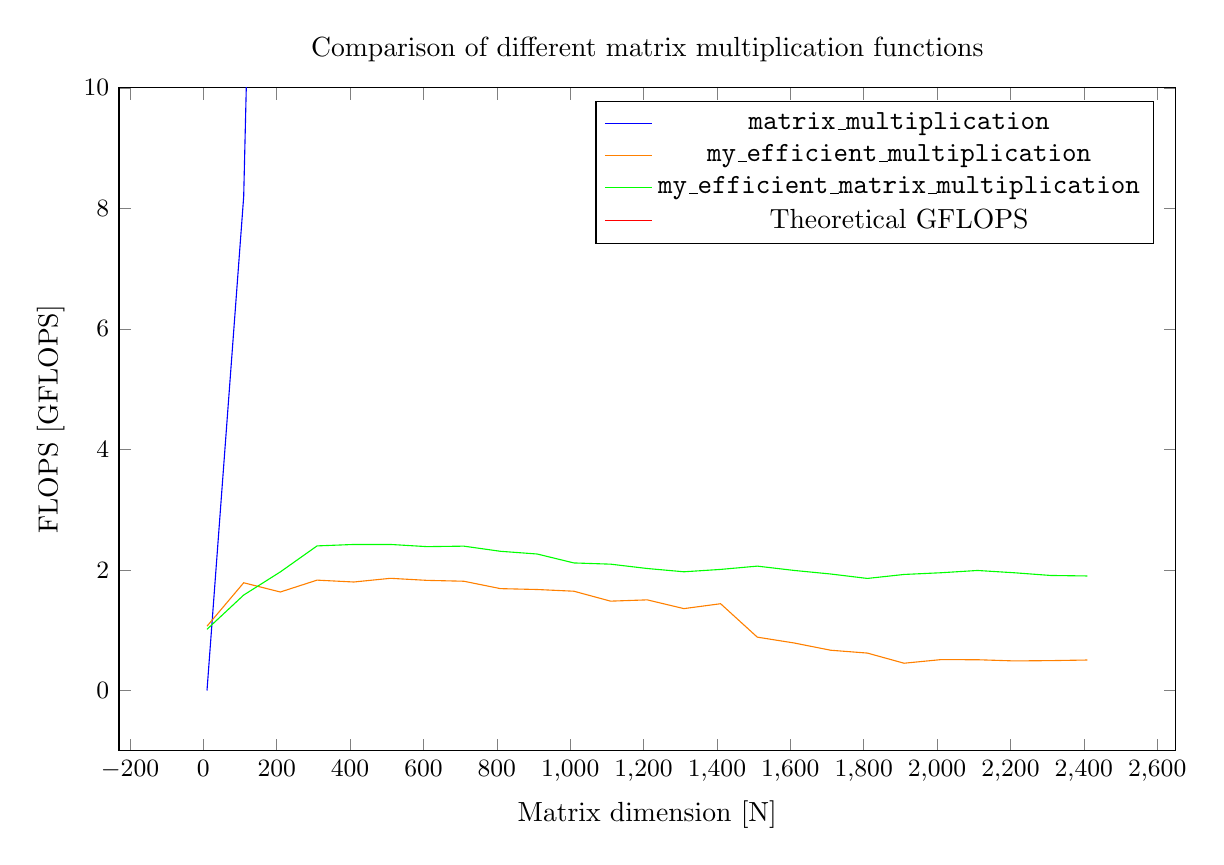
\begin{tikzpicture}
\begin{axis}[width={15cm}, height={10cm}, xlabel={Matrix dimension [N]}, ylabel={FLOPS [GFLOPS]}, title={Comparison of different matrix multiplication functions}, legend={north east}, ymax={10},    scaled ticks=false,   % Prevents scientific notation or compression in the ticks
    xticklabel style={/pgf/number format/fixed},  % Ensures tick labels are printed in a fixed format without rounding
    xticklabel style={/pgf/number format/precision=0},  % Rounds the numbers to integers to avoid crowding
    ticklabel style = {font=\small},  % Reduces the size of the tick labels to prevent overlap
    ]
    \addplot[no marks, blue]
        table[row sep={\\}]
        {
            \\
            10.0  0.0023079523961738765  \\
            110.0  8.194097294901313  \\
            210.0  33.72498893859692  \\
            310.0  63.67891003491642  \\
            410.0  83.20933205921395  \\
            510.0  121.0965154318156  \\
            610.0  114.15410635879024  \\
            710.0  148.78480554332117  \\
            810.0  128.77979771936313  \\
            910.0  46.69649114974178  \\
            1010.0  149.39668260804913  \\
            1110.0  185.67318648613312  \\
            1210.0  139.70476585037548  \\
            1310.0  140.825722756572  \\
            1410.0  157.08443564188434  \\
            1510.0  189.98083748640684  \\
            1610.0  201.73749401185015  \\
            1710.0  238.16347699049706  \\
            1810.0  184.7190920582196  \\
            1910.0  236.60746961674465  \\
            2010.0  189.07665556113673  \\
            2110.0  208.35783211953395  \\
            2210.0  211.28693733594844  \\
            2310.0  220.6979894130633  \\
            2410.0  185.3414228183199  \\
        }
        ;
    \addplot[no marks, orange]
        table[row sep={\\}]
        {
            \\
            10.0  1.0689470871191875  \\
            110.0  1.7891119566042895  \\
            210.0  1.6363952973381144  \\
            310.0  1.833138380472606  \\
            410.0  1.8019750452823982  \\
            510.0  1.8633233611285047  \\
            610.0  1.829149502012656  \\
            710.0  1.814902720882529  \\
            810.0  1.691969911709576  \\
            910.0  1.67758644720142  \\
            1010.0  1.649210445467428  \\
            1110.0  1.4844659134712057  \\
            1210.0  1.50570400213252  \\
            1310.0  1.36048195288819  \\
            1410.0  1.441815509625949  \\
            1510.0  0.8870844660154257  \\
            1610.0  0.7907230876381947  \\
            1710.0  0.6699917469778933  \\
            1810.0  0.622945715952708  \\
            1910.0  0.4545396698327844  \\
            2010.0  0.5141040422999137  \\
            2110.0  0.5125469619014145  \\
            2210.0  0.49265788054693666  \\
            2310.0  0.497771062036038  \\
            2410.0  0.5078183160369875  \\
        }
        ;
    \addplot[no marks, green]
        table[row sep={\\}]
        {
            \\
            10.0  1.017293997965412  \\
            110.0  1.5855298659744814  \\
            210.0  1.9699571431686191  \\
            310.0  2.4009089137903974  \\
            410.0  2.424738077028364  \\
            510.0  2.4250974800940805  \\
            610.0  2.3888349809526823  \\
            710.0  2.3969416901613645  \\
            810.0  2.3114564185518116  \\
            910.0  2.2665805230657363  \\
            1010.0  2.1183366990174863  \\
            1110.0  2.098103432813833  \\
            1210.0  2.02596145383276  \\
            1310.0  1.9715949457443354  \\
            1410.0  2.010909758662662  \\
            1510.0  2.065411932336678  \\
            1610.0  1.9941957000538721  \\
            1710.0  1.9348035190308683  \\
            1810.0  1.86114085663287  \\
            1910.0  1.9272390772083445  \\
            2010.0  1.9553976471457613  \\
            2110.0  1.993427896663581  \\
            2210.0  1.9556294361633033  \\
            2310.0  1.9104629902084065  \\
            2410.0  1.9020792743764794  \\
        }
        ;
    \addplot[no marks, red]
        table[row sep={\\}]
        {
            \\
            10.0  288.0  \\
            110.0  288.0  \\
            210.0  288.0  \\
            310.0  288.0  \\
            410.0  288.0  \\
            510.0  288.0  \\
            610.0  288.0  \\
            710.0  288.0  \\
            810.0  288.0  \\
            910.0  288.0  \\
            1010.0  288.0  \\
            1110.0  288.0  \\
            1210.0  288.0  \\
            1310.0  288.0  \\
            1410.0  288.0  \\
            1510.0  288.0  \\
            1610.0  288.0  \\
            1710.0  288.0  \\
            1810.0  288.0  \\
            1910.0  288.0  \\
            2010.0  288.0  \\
            2110.0  288.0  \\
            2210.0  288.0  \\
            2310.0  288.0  \\
            2410.0  288.0  \\
        }
        ;
        \addlegendentry {\texttt{matrix\_multiplication}}
        \addlegendentry {\texttt{my\_efficient\_multiplication}}
        \addlegendentry {\texttt{my\_efficient\_matrix\_multiplication}}
        \addlegendentry {Theoretical GFLOPS}        
\end{axis}
\end{tikzpicture}

     \end{center}
     \caption{Matrix product efficiency, tested on a Intel(R) Core(TM) i7-8557U CPU @ 1.70GHz (2)}
     \label{fig:2-dotproductcomparison}
 \end{figure}

\clearpage
\newpage


\subsection{Comparison of BLAS Operations Across Different Levels}
But what about matrix-vector multiplications? It is logical to consider the optimal shape and dimensions of these matrices. 
One might intuitively assume that a matrix-vector multiplication is faster than a matrix-matrix multiplication.
To visualize the load that the CPU experiences in both cases, the following code is used to plot the figures.

\vspace*{0.5cm}

\lstinputlisting[language=Julia]{code/BLAS_levels.jl}

\vspace*{0.5cm}

\begin{figure}[h]
\begin{center}
    % Recommended preamble:
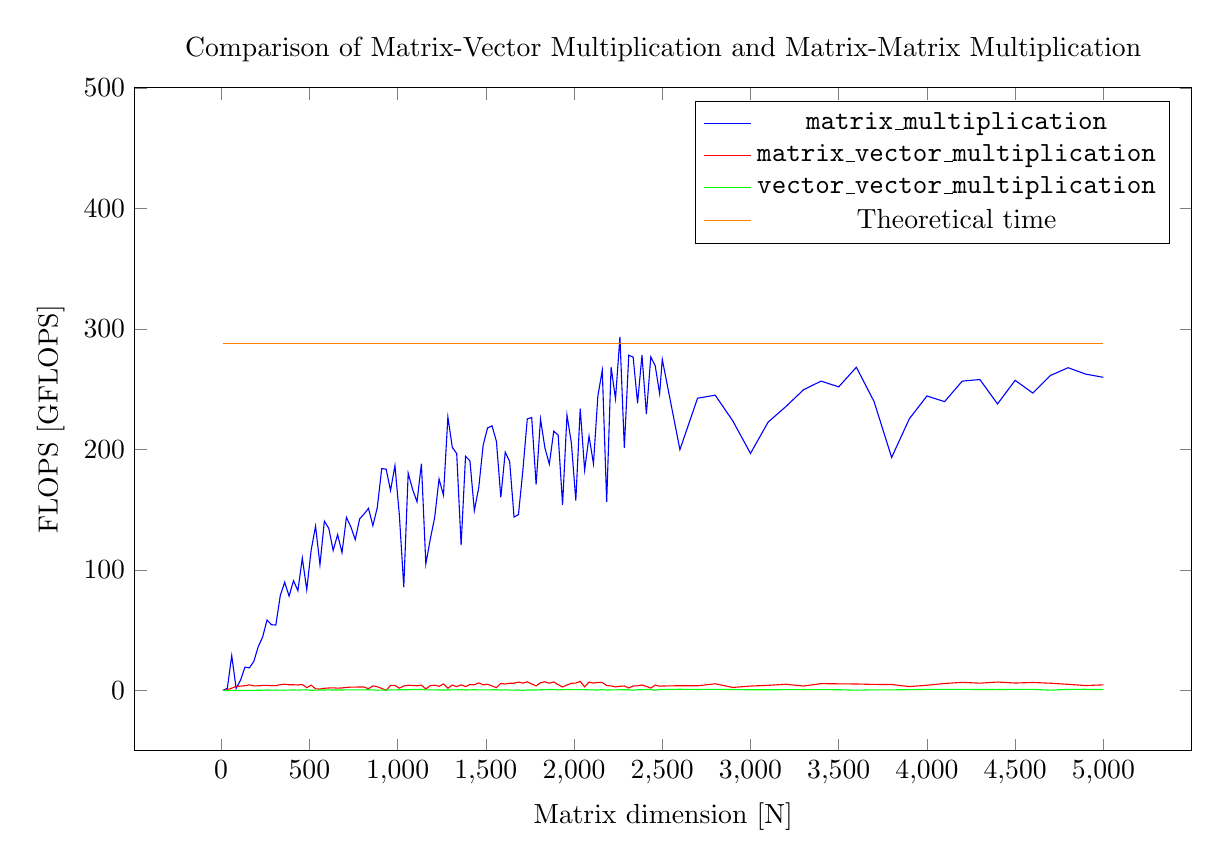
\begin{tikzpicture}
\begin{axis}[width={15cm}, height={10cm}, xlabel={Matrix dimension [N]}, ylabel={FLOPS [GFLOPS]}, title={Comparison of Matrix-Vector Multiplication and Matrix-Matrix Multiplication}, legend={north east}, ymax={500}]
    \addplot[no marks, blue]
        table[row sep={\\}]
        {
            \\
            10.0  0.00023735286051140286  \\
            35.0  1.8266445126107702  \\
            60.0  28.92728003214142  \\
            85.0  1.6462358731316078  \\
            110.0  8.66341869827415  \\
            135.0  19.369447385719965  \\
            160.0  18.755136943178254  \\
            185.0  24.092712207836684  \\
            210.0  36.257857141458885  \\
            235.0  44.314565420784135  \\
            260.0  58.44075957027288  \\
            285.0  54.576140719819314  \\
            310.0  54.29418111303892  \\
            335.0  78.69009868868586  \\
            360.0  89.8249072746893  \\
            385.0  78.31813287970999  \\
            410.0  91.11580873361176  \\
            435.0  82.77338472592267  \\
            460.0  109.91630591956493  \\
            485.0  83.6076671790578  \\
            510.0  116.31012526150948  \\
            535.0  136.3508365303236  \\
            560.0  104.29141449863026  \\
            585.0  140.48561525288082  \\
            610.0  134.55378496801708  \\
            635.0  116.21255795925332  \\
            660.0  129.30891407336844  \\
            685.0  114.43687076149929  \\
            710.0  143.64748649708972  \\
            735.0  135.7695713208871  \\
            760.0  125.21616301012152  \\
            785.0  142.40380890308208  \\
            810.0  146.4390285839937  \\
            835.0  151.08798486895742  \\
            860.0  136.79613589241458  \\
            885.0  151.83550320744158  \\
            910.0  184.10195477821713  \\
            935.0  183.68331047779773  \\
            960.0  165.89797980034737  \\
            985.0  186.63288902307468  \\
            1010.0  145.5539478662233  \\
            1035.0  85.84116813955796  \\
            1060.0  180.31715559942725  \\
            1085.0  166.8072682514341  \\
            1110.0  156.5568485028589  \\
            1135.0  188.11624237215517  \\
            1160.0  104.95485127794238  \\
            1185.0  125.42631303170059  \\
            1210.0  143.3921637808318  \\
            1235.0  175.4632141674464  \\
            1260.0  162.0556196725115  \\
            1285.0  226.89372516272846  \\
            1310.0  201.79996849247254  \\
            1335.0  196.53080970413205  \\
            1360.0  120.54266472715214  \\
            1385.0  194.33739426070323  \\
            1410.0  190.50246449503956  \\
            1435.0  149.27629620095067  \\
            1460.0  168.48990456887893  \\
            1485.0  203.62494767542074  \\
            1510.0  217.84711470582596  \\
            1535.0  219.56858219147125  \\
            1560.0  206.84355955322113  \\
            1585.0  160.34243896137565  \\
            1610.0  197.72951864087614  \\
            1635.0  189.9645287963804  \\
            1660.0  143.88657212456386  \\
            1685.0  145.95230940426606  \\
            1710.0  182.71589356195926  \\
            1735.0  225.33715315261833  \\
            1760.0  226.5185839605248  \\
            1785.0  170.93730928923088  \\
            1810.0  225.17261440412383  \\
            1835.0  201.19296185498513  \\
            1860.0  187.86489412050884  \\
            1885.0  215.16034520656507  \\
            1910.0  211.9352634672822  \\
            1935.0  154.12981763154013  \\
            1960.0  228.4821628792833  \\
            1985.0  205.25343700293823  \\
            2010.0  157.60220556890428  \\
            2035.0  233.90041455368387  \\
            2060.0  182.87409933734776  \\
            2085.0  211.02988778492522  \\
            2110.0  188.1566760543063  \\
            2135.0  244.26527954650308  \\
            2160.0  265.7174692898608  \\
            2185.0  156.5263302218174  \\
            2210.0  268.2479682949384  \\
            2235.0  242.02406286743764  \\
            2260.0  293.40068847583615  \\
            2285.0  201.2885254632914  \\
            2310.0  278.15430681461964  \\
            2335.0  276.62191232583945  \\
            2360.0  238.34265072537647  \\
            2385.0  278.18471215461506  \\
            2410.0  229.24491546677055  \\
            2435.0  276.83255957868005  \\
            2460.0  269.43063227706887  \\
            2485.0  246.2499101261397  \\
            2500.0  274.7579123420797  \\
            2600.0  199.8495783982345  \\
            2700.0  242.49924205896602  \\
            2800.0  245.01651263628966  \\
            2900.0  223.6033542556816  \\
            3000.0  196.72210624705218  \\
            3100.0  222.71242812611638  \\
            3200.0  235.508416371348  \\
            3300.0  249.4599823414236  \\
            3400.0  256.6880799584675  \\
            3500.0  251.92273749687772  \\
            3600.0  268.19559000362557  \\
            3700.0  239.8471743599322  \\
            3800.0  193.3464055099314  \\
            3900.0  225.37951408805193  \\
            4000.0  244.35539841008978  \\
            4100.0  239.66615698125284  \\
            4200.0  256.69404704164407  \\
            4300.0  258.0059741848452  \\
            4400.0  237.78058288125905  \\
            4500.0  257.3327020518556  \\
            4600.0  246.76345865474775  \\
            4700.0  261.37674684881256  \\
            4800.0  267.80212423297974  \\
            4900.0  262.4908914161355  \\
            5000.0  259.8166895771811  \\
        }
        ;
    \addplot[no marks, red]
        table[row sep={\\}]
        {
            \\
            10.0  0.04038772213247173  \\
            35.0  0.6474630021141649  \\
            60.0  1.9072847682119205  \\
            85.0  3.369869402985075  \\
            110.0  3.6309077269317327  \\
            135.0  3.977520733304234  \\
            160.0  4.690792487402657  \\
            185.0  3.826373749231371  \\
            210.0  3.871987356775978  \\
            235.0  4.203615604186489  \\
            260.0  4.292472298949106  \\
            285.0  3.9647093278664514  \\
            310.0  4.018398494668618  \\
            335.0  4.833326155303847  \\
            360.0  5.184518451845184  \\
            385.0  4.729805191697114  \\
            410.0  4.763591538319849  \\
            435.0  4.552343834578327  \\
            460.0  4.951039460907612  \\
            485.0  2.34843379508299  \\
            510.0  4.421514296399551  \\
            535.0  1.3554534239731395  \\
            560.0  1.1552835989147112  \\
            585.0  1.8188509974515623  \\
            610.0  2.08815012682664  \\
            635.0  2.189007326096811  \\
            660.0  1.939214787180526  \\
            685.0  2.1015281398077734  \\
            710.0  2.5428837340691435  \\
            735.0  2.7973250069904  \\
            760.0  2.7996568287682186  \\
            785.0  2.9174626395763648  \\
            810.0  2.8470075178182057  \\
            835.0  1.471997787437798  \\
            860.0  3.8074450067181123  \\
            885.0  3.0598013458476983  \\
            910.0  1.7348021506435067  \\
            935.0  0.11851605923274638  \\
            960.0  4.204955057717753  \\
            985.0  4.164529442189777  \\
            1010.0  1.914215881743079  \\
            1035.0  3.756292045592018  \\
            1060.0  4.3230182639441965  \\
            1085.0  4.153626583774667  \\
            1110.0  3.9032379673130353  \\
            1135.0  4.476096330450555  \\
            1160.0  1.2727755985762619  \\
            1185.0  3.9994218286733103  \\
            1210.0  4.445929018789144  \\
            1235.0  3.4416056952992347  \\
            1260.0  5.430356431274831  \\
            1285.0  1.7928269549709968  \\
            1310.0  4.532877958844606  \\
            1335.0  3.1668770839978286  \\
            1360.0  4.668967998031037  \\
            1385.0  3.2287724276998873  \\
            1410.0  4.963270400998596  \\
            1435.0  4.711894230791232  \\
            1460.0  6.246025908876471  \\
            1485.0  4.715581106669247  \\
            1510.0  5.15222112001663  \\
            1535.0  3.754623115497815  \\
            1560.0  2.3816490884339894  \\
            1585.0  5.914861406396048  \\
            1610.0  5.3791456162795885  \\
            1635.0  6.012496302952128  \\
            1660.0  6.007942711314167  \\
            1685.0  6.9813860850535425  \\
            1710.0  6.123596505648531  \\
            1735.0  7.2196999131782045  \\
            1760.0  5.33927658800645  \\
            1785.0  3.832358772937952  \\
            1810.0  6.435296405497728  \\
            1835.0  7.2067516779672625  \\
            1860.0  6.040874910620509  \\
            1885.0  7.117132816357352  \\
            1910.0  4.81206359716956  \\
            1935.0  2.8951521487325964  \\
            1960.0  4.562245447522479  \\
            1985.0  5.953773252765552  \\
            2010.0  6.166481727671097  \\
            2035.0  7.578540043664366  \\
            2060.0  3.0203590964687863  \\
            2085.0  6.945680464107853  \\
            2110.0  6.1668645134838265  \\
            2135.0  6.675974196685465  \\
            2160.0  6.568251760459282  \\
            2185.0  4.150951352516885  \\
            2210.0  3.761134354609798  \\
            2235.0  2.9333378354175044  \\
            2260.0  3.48676624890006  \\
            2285.0  3.7088714641241993  \\
            2310.0  2.083170263379853  \\
            2335.0  3.720556900437243  \\
            2360.0  3.86289684665799  \\
            2385.0  4.510773327539133  \\
            2410.0  3.4254466553961507  \\
            2435.0  1.9768722393521678  \\
            2460.0  4.487940828240002  \\
            2485.0  3.5444291639354986  \\
            2500.0  3.7150182734318835  \\
            2600.0  3.960732501149843  \\
            2700.0  3.8824020938343033  \\
            2800.0  5.553367579100072  \\
            2900.0  2.5307553733037205  \\
            3000.0  3.672333962050509  \\
            3100.0  4.267501752961828  \\
            3200.0  5.159863817891072  \\
            3300.0  3.6895337008750357  \\
            3400.0  5.682082099696456  \\
            3500.0  5.527524363973717  \\
            3600.0  5.382689047743746  \\
            3700.0  5.019562176114034  \\
            3800.0  4.976975456858946  \\
            3900.0  3.2288561665580295  \\
            4000.0  4.355687629683794  \\
            4100.0  5.800819326908262  \\
            4200.0  6.761830616143066  \\
            4300.0  6.065022353494366  \\
            4400.0  7.012545247850552  \\
            4500.0  6.178148514147655  \\
            4600.0  6.6362328276498825  \\
            4700.0  6.034111990550837  \\
            4800.0  5.080672209979948  \\
            4900.0  4.090876060000765  \\
            5000.0  4.679102035400027  \\
        }
        ;
    \addplot[no marks, green]
        table[row sep={\\}]
        {
            \\
            10.0  0.0032674399607907204  \\
            35.0  0.020958083832335328  \\
            60.0  0.046838407494145196  \\
            85.0  0.07834101382488479  \\
            110.0  0.08644400785854617  \\
            135.0  0.10424710424710423  \\
            160.0  0.14890646812470917  \\
            185.0  0.11824864173857462  \\
            210.0  0.1972757162987318  \\
            235.0  0.23653749370910923  \\
            260.0  0.47619047619047616  \\
            285.0  0.29290853031860226  \\
            310.0  0.38969201759899436  \\
            335.0  0.2571976967370442  \\
            360.0  0.23323615160349856  \\
            385.0  0.3389084507042253  \\
            410.0  0.4017638412542871  \\
            435.0  0.31487513572204123  \\
            460.0  0.46605876393110435  \\
            485.0  0.6123737373737373  \\
            510.0  0.07051991150442478  \\
            535.0  0.2859433458043827  \\
            560.0  0.3604763437399421  \\
            585.0  0.412407472682411  \\
            610.0  0.47470817120622566  \\
            635.0  0.4191419141914191  \\
            660.0  0.3880070546737214  \\
            685.0  0.430411561420044  \\
            710.0  0.46103896103896097  \\
            735.0  0.448444173276388  \\
            760.0  0.5594405594405594  \\
            785.0  0.5516514406184118  \\
            810.0  0.5465587044534412  \\
            835.0  0.5831005586592178  \\
            860.0  0.5041031652989448  \\
            885.0  0.22859356838434716  \\
            910.0  0.2720885035132307  \\
            935.0  0.3410541674265913  \\
            960.0  0.5010438413361169  \\
            985.0  0.5093071354705274  \\
            1010.0  0.618304254667891  \\
            1035.0  0.5569007263922517  \\
            1060.0  0.6257378984651712  \\
            1085.0  0.8420644159875824  \\
            1110.0  0.847651775486827  \\
            1135.0  0.8657513348588863  \\
            1160.0  0.4597701149425288  \\
            1185.0  0.484167517875383  \\
            1210.0  0.46772323154232703  \\
            1235.0  0.4209988068859724  \\
            1260.0  0.4190919674039581  \\
            1285.0  0.35585710329548603  \\
            1310.0  0.5059868675164156  \\
            1335.0  0.5519950382468473  \\
            1360.0  0.690180157320477  \\
            1385.0  0.35259674134419555  \\
            1410.0  0.5380652547223812  \\
            1435.0  0.5948186528497409  \\
            1460.0  0.5394420838721596  \\
            1485.0  0.4638450726222083  \\
            1510.0  0.4946764946764947  \\
            1535.0  0.5824321760576741  \\
            1560.0  0.6439628482972136  \\
            1585.0  0.3203314470493128  \\
            1610.0  0.5905006418485237  \\
            1635.0  0.31202290076335876  \\
            1660.0  0.31907736665064873  \\
            1685.0  0.4763250883392226  \\
            1710.0  0.0909526089037817  \\
            1735.0  0.4149724946185123  \\
            1760.0  0.44915146101824677  \\
            1785.0  0.4031620553359684  \\
            1810.0  0.6237077877325983  \\
            1835.0  0.6719150494324423  \\
            1860.0  0.7993124194241513  \\
            1885.0  0.8176100628930817  \\
            1910.0  0.5247252747252747  \\
            1935.0  0.6116642958748222  \\
            1960.0  0.920836269673479  \\
            1985.0  0.7245847782442052  \\
            2010.0  0.7545045045045046  \\
            2035.0  0.7394622093023255  \\
            2060.0  0.6646233263429585  \\
            2085.0  0.5122850122850122  \\
            2110.0  0.46573225913254607  \\
            2135.0  0.3538869550803912  \\
            2160.0  0.8121827411167513  \\
            2185.0  0.34918098282061527  \\
            2210.0  0.4482758620689655  \\
            2235.0  0.45926230350354463  \\
            2260.0  0.6781695423855965  \\
            2285.0  0.5805386178861789  \\
            2310.0  0.6193029490616622  \\
            2335.0  0.182486030245008  \\
            2360.0  0.6398264877321405  \\
            2385.0  0.6531562371628098  \\
            2410.0  0.8423628102062216  \\
            2435.0  0.7975761546020308  \\
            2460.0  0.09568447461055252  \\
            2485.0  0.8577839143942009  \\
            2500.0  0.8305647840531561  \\
            2600.0  0.9967414222733372  \\
            2700.0  0.8478568064060291  \\
            2800.0  0.9362982778799532  \\
            2900.0  0.821297082979326  \\
            3000.0  0.5694760820045558  \\
            3100.0  0.6203722233340004  \\
            3200.0  0.67425200168563  \\
            3300.0  0.7806031933767003  \\
            3400.0  0.6726679196755366  \\
            3500.0  0.6440334897414666  \\
            3600.0  0.23203351595230426  \\
            3700.0  0.5489614243323442  \\
            3800.0  0.5302078973071019  \\
            3900.0  0.6821163095758637  \\
            4000.0  0.887606790191945  \\
            4100.0  0.8935381933093604  \\
            4200.0  0.9595613433858808  \\
            4300.0  0.7872574148663494  \\
            4400.0  0.7692980155608008  \\
            4500.0  0.9266886326194399  \\
            4600.0  0.9240658899156288  \\
            4700.0  0.2673340538080883  \\
            4800.0  0.9374084562054488  \\
            4900.0  0.9862131427996377  \\
            5000.0  0.7254788160185722  \\
        }
        ;
    \addplot[no marks, orange]
        table[row sep={\\}]
        {
            \\
            10.0  288.0  \\
            35.0  288.0  \\
            60.0  288.0  \\
            85.0  288.0  \\
            110.0  288.0  \\
            135.0  288.0  \\
            160.0  288.0  \\
            185.0  288.0  \\
            210.0  288.0  \\
            235.0  288.0  \\
            260.0  288.0  \\
            285.0  288.0  \\
            310.0  288.0  \\
            335.0  288.0  \\
            360.0  288.0  \\
            385.0  288.0  \\
            410.0  288.0  \\
            435.0  288.0  \\
            460.0  288.0  \\
            485.0  288.0  \\
            510.0  288.0  \\
            535.0  288.0  \\
            560.0  288.0  \\
            585.0  288.0  \\
            610.0  288.0  \\
            635.0  288.0  \\
            660.0  288.0  \\
            685.0  288.0  \\
            710.0  288.0  \\
            735.0  288.0  \\
            760.0  288.0  \\
            785.0  288.0  \\
            810.0  288.0  \\
            835.0  288.0  \\
            860.0  288.0  \\
            885.0  288.0  \\
            910.0  288.0  \\
            935.0  288.0  \\
            960.0  288.0  \\
            985.0  288.0  \\
            1010.0  288.0  \\
            1035.0  288.0  \\
            1060.0  288.0  \\
            1085.0  288.0  \\
            1110.0  288.0  \\
            1135.0  288.0  \\
            1160.0  288.0  \\
            1185.0  288.0  \\
            1210.0  288.0  \\
            1235.0  288.0  \\
            1260.0  288.0  \\
            1285.0  288.0  \\
            1310.0  288.0  \\
            1335.0  288.0  \\
            1360.0  288.0  \\
            1385.0  288.0  \\
            1410.0  288.0  \\
            1435.0  288.0  \\
            1460.0  288.0  \\
            1485.0  288.0  \\
            1510.0  288.0  \\
            1535.0  288.0  \\
            1560.0  288.0  \\
            1585.0  288.0  \\
            1610.0  288.0  \\
            1635.0  288.0  \\
            1660.0  288.0  \\
            1685.0  288.0  \\
            1710.0  288.0  \\
            1735.0  288.0  \\
            1760.0  288.0  \\
            1785.0  288.0  \\
            1810.0  288.0  \\
            1835.0  288.0  \\
            1860.0  288.0  \\
            1885.0  288.0  \\
            1910.0  288.0  \\
            1935.0  288.0  \\
            1960.0  288.0  \\
            1985.0  288.0  \\
            2010.0  288.0  \\
            2035.0  288.0  \\
            2060.0  288.0  \\
            2085.0  288.0  \\
            2110.0  288.0  \\
            2135.0  288.0  \\
            2160.0  288.0  \\
            2185.0  288.0  \\
            2210.0  288.0  \\
            2235.0  288.0  \\
            2260.0  288.0  \\
            2285.0  288.0  \\
            2310.0  288.0  \\
            2335.0  288.0  \\
            2360.0  288.0  \\
            2385.0  288.0  \\
            2410.0  288.0  \\
            2435.0  288.0  \\
            2460.0  288.0  \\
            2485.0  288.0  \\
            2500.0  288.0  \\
            2600.0  288.0  \\
            2700.0  288.0  \\
            2800.0  288.0  \\
            2900.0  288.0  \\
            3000.0  288.0  \\
            3100.0  288.0  \\
            3200.0  288.0  \\
            3300.0  288.0  \\
            3400.0  288.0  \\
            3500.0  288.0  \\
            3600.0  288.0  \\
            3700.0  288.0  \\
            3800.0  288.0  \\
            3900.0  288.0  \\
            4000.0  288.0  \\
            4100.0  288.0  \\
            4200.0  288.0  \\
            4300.0  288.0  \\
            4400.0  288.0  \\
            4500.0  288.0  \\
            4600.0  288.0  \\
            4700.0  288.0  \\
            4800.0  288.0  \\
            4900.0  288.0  \\
            5000.0  288.0  \\
        }
        ;
    \addlegendentry {\texttt{matrix\_multiplication}}
    \addlegendentry {\texttt{matrix\_vector\_multiplication}}
    \addlegendentry {{\texttt{vector\_vector\_multiplication}}}
    \addlegendentry {Theoretical time}
\end{axis}
\end{tikzpicture}

\end{center}
    \caption{Representation of GFLOPS for the different levels of BLAS: matrix multiplication (Level 3 BLAS), 
    matrix-vector multiplication (Level 2 BLAS), and vector multiplication (dot product, Level 1 BLAS).}
    \label{fig:matvec_vs_matmul}
\end{figure}

\newpage

\paragraph*{} Figure \ref{fig:matvec_vs_matmul} illustrates the inherent limitation in matrix-vector multiplication 
(which is not due to CPU capacity but rather a bottleneck issue). This limitation arises because the ``usability'' of data in a matrix-matrix operation is higher than in a matrix-vector operation. 
Consider the following example with $N$:

\begin{equation}
    \begin{bmatrix}
        a_{11} & \hdots & a_{1N} \\
        \vdots & \ddots & \vdots \\
        a_{N1} & \hdots & a_{NN} 
    \end{bmatrix}
    \begin{bmatrix}
        b_{11} & \hdots & b_{1N} \\
        \vdots & \ddots & \vdots \\
        b_{N1} & \hdots & b_{NN} 
    \end{bmatrix}
    =
    \begin{bmatrix}
        c_{11} & \hdots & c_{1N} \\
        \vdots & \ddots & \vdots \\
        c_{N1} & \hdots & c_{NN} 
    \end{bmatrix}
    \label{eq_matrix1}
\end{equation}

\vspace{0.5cm}

\begin{equation}
    \begin{bmatrix}
        \alpha_{11} & \hdots & \alpha_{1N} \\
        \vdots & \ddots & \vdots \\
        \alpha_{N1} & \hdots & \alpha_{NN} 
    \end{bmatrix}
    \begin{bmatrix}
        \beta_{1} \\
        \vdots \\
        \beta_{N}
    \end{bmatrix}
    =
    \begin{bmatrix}
        \gamma_{1} \\
        \vdots \\
        \gamma_{N}
    \end{bmatrix}
    \label{eq_matrix2}
\end{equation}

\vspace{0.5cm}

\paragraph*{} In this example, vector $\vec{a}_1 = \sum_{i=1}^{N} a_{1i} \vec{e}_i$ is used $N$ times to compute $N$ values ($\sum_{i=1}^{N} c_{i1} \vec{e}_i$). 
In contrast, the vector of elements $\vec{\alpha}_1 = \sum_{i=1}^{N} \alpha_{1i} \vec{e}_i$ is only used once (to compute $\gamma_{1}$).

\paragraph*{} We can define the term "usability" as the ratio between the number of operations performed by the CPU and the number 
of data elements (in this case, Float32) used during the process. This can be expressed as:

\begin{equation}
    U = \frac{N_{ops}}{N_{data}}
\end{equation}

where $N_{ops}$ represents the number of operations executed by the CPU, and $N_{data}$ denotes the number of data elements 
involved in the process.

\paragraph*{} For matrix multiplication of dimension $N$, considering the use of Fused Multiply-Add (FMA), we have $N_{ops} = N^3$ 
and $N_{data} = 2N^2$. This yields a usability value greater than 1.

\paragraph*{} In the case of matrix-vector multiplication, again with dimension $N$ (as shown in expression \ref{eq_matrix2}),
$N_{ops} = N^2$ and $N_{data} = N^2 + N$. Here, the usability value is approximately 1.

\paragraph*{Scalar product} It is worth noting that the graph \ref{fig:matvec_vs_matmul} also includes the vector-vector product.
As expected, the results are even worse. The value of \textbf{U} is less than 1 ($N_{ops} = N$ and $N_{data} = 2N$)

\paragraph*{} In conclusion, \textbf{as the usability value tends towards infinity, and with sufficiently large values of N, the CPU's 
performance approaches its theoretical maximum.}

%!!! NOTE !!! For including .tex files that makes some graphics from a .jl file, use this:
% \begin{tikzpicture}
% \begin{axis}[xlabel={x}, ylabel={y}, title={Gráfico de ejemplo}]
%    \addplot[no marks]
%       table[row sep={\\}]
%       {
%           .
%           .
%           .
%        }
%       ;
% \end{axis}
% \end{tikzpicture}
\clearpage
\newpage